%!TEX root = ../thesis.tex
\documentclass[../thesis]{subfiles}

\begin{document}
	\section{Strategies}
	\label{sec:case:strategy}

	\tdg{dependencies}%
	\Cref{eq:sqrtm:diag0,eq:sqrtm:diagN} describe an algorithm where each element depends on those at its left in the same row and those below in the same column (Parlett's recurrence \cite{Parlett:1976}). Consequently, the algorithm can be implemented either a column/row or a superdiagonal at a time.

	% \subfile{tex/fig/dependencies.tex}

	\tdg{column/row}%
	While the first strategy (column/row) is preferred for any serial implementation due to a more efficient use of cache memory (better locality), it presents almost\footnote{It is possible for this strategy to solve its dependencies in parallel. The following chapters will show this with more detail.} no opportunities for parallelism since no more than one element is ready to be computed at any given time.

	\tdg{super-diagonal}%
	On the other hand, computing a super-diagonal at a time allows for several elements to be computed in parallel since all the dependencies were already computed in previous super-diagonals.

	\begin{figure}[htp]
		\addtolength\belowcaptionskip{1cm}
		\begin{subfigure}{\textwidth}
			\centering
			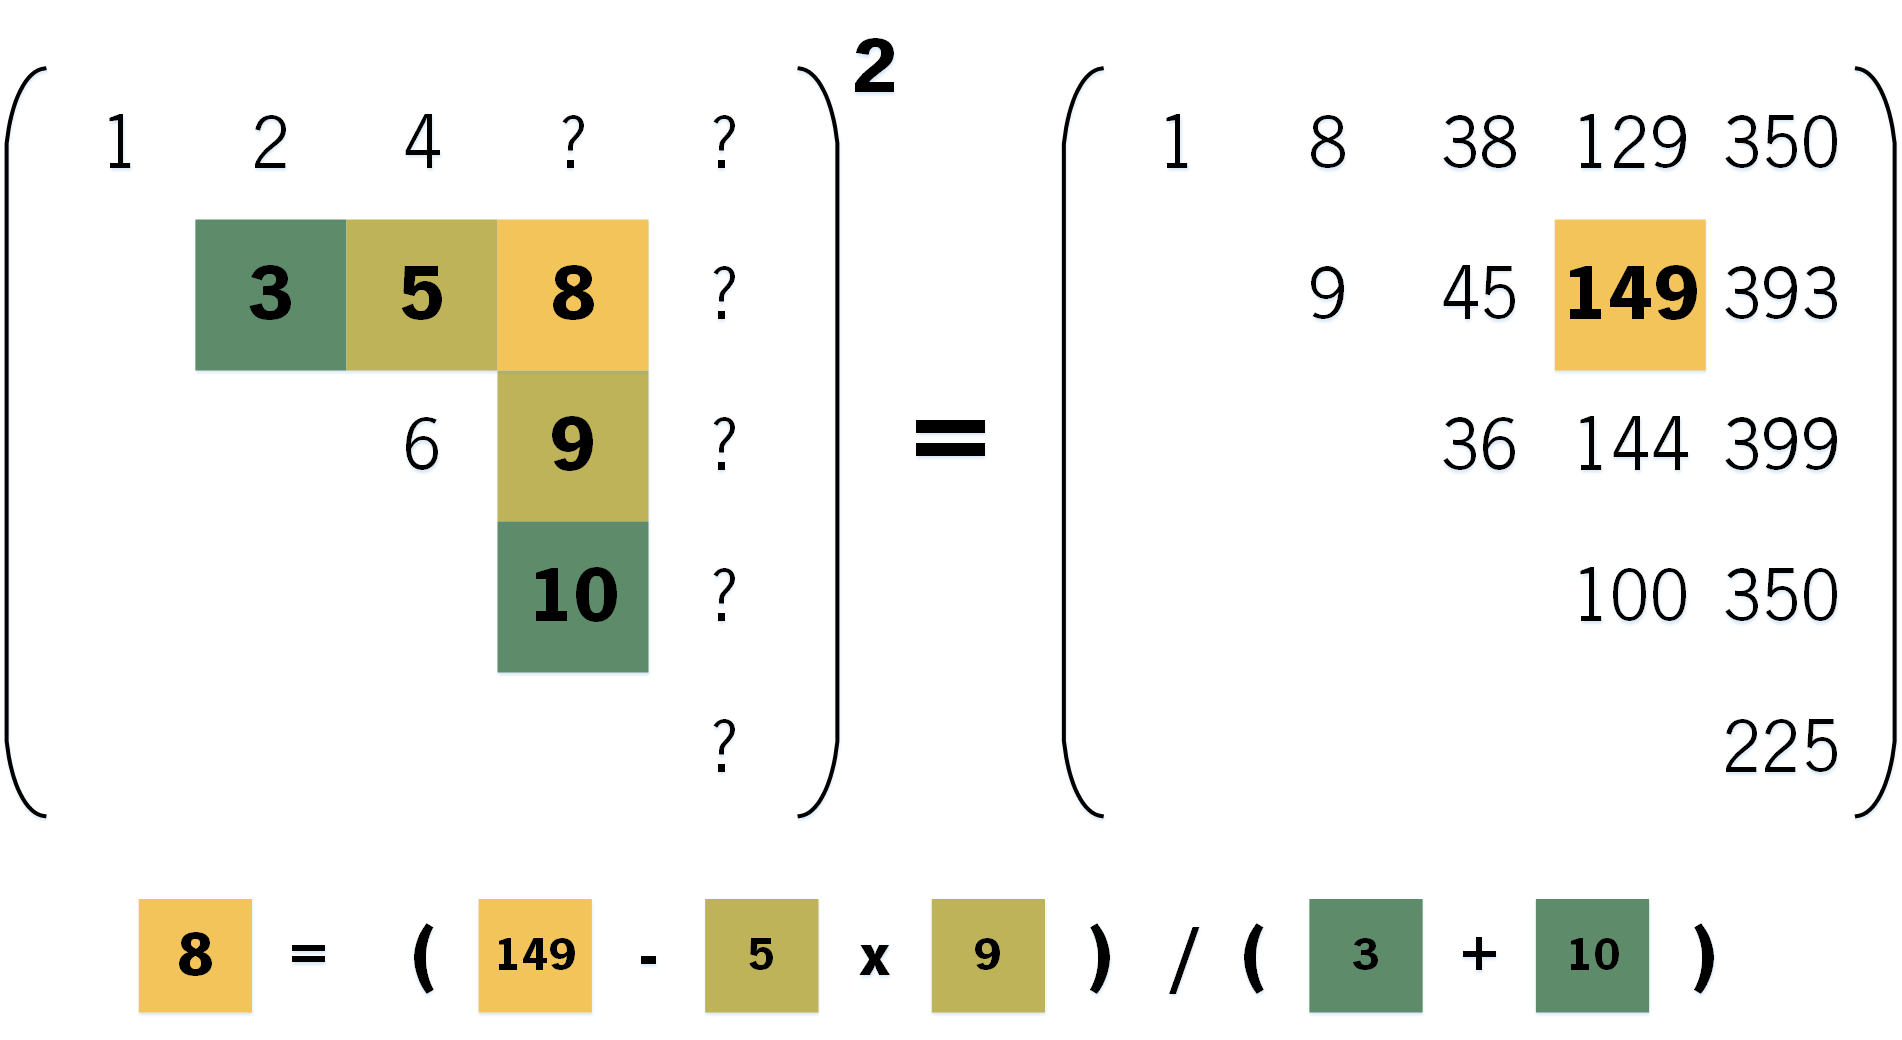
\includegraphics[height=0.2\textheight]{assets/images/case/dependencies.png}
			\caption{Dependencies}
		\end{subfigure}
		\begin{subfigure}{\textwidth}
			\centering
			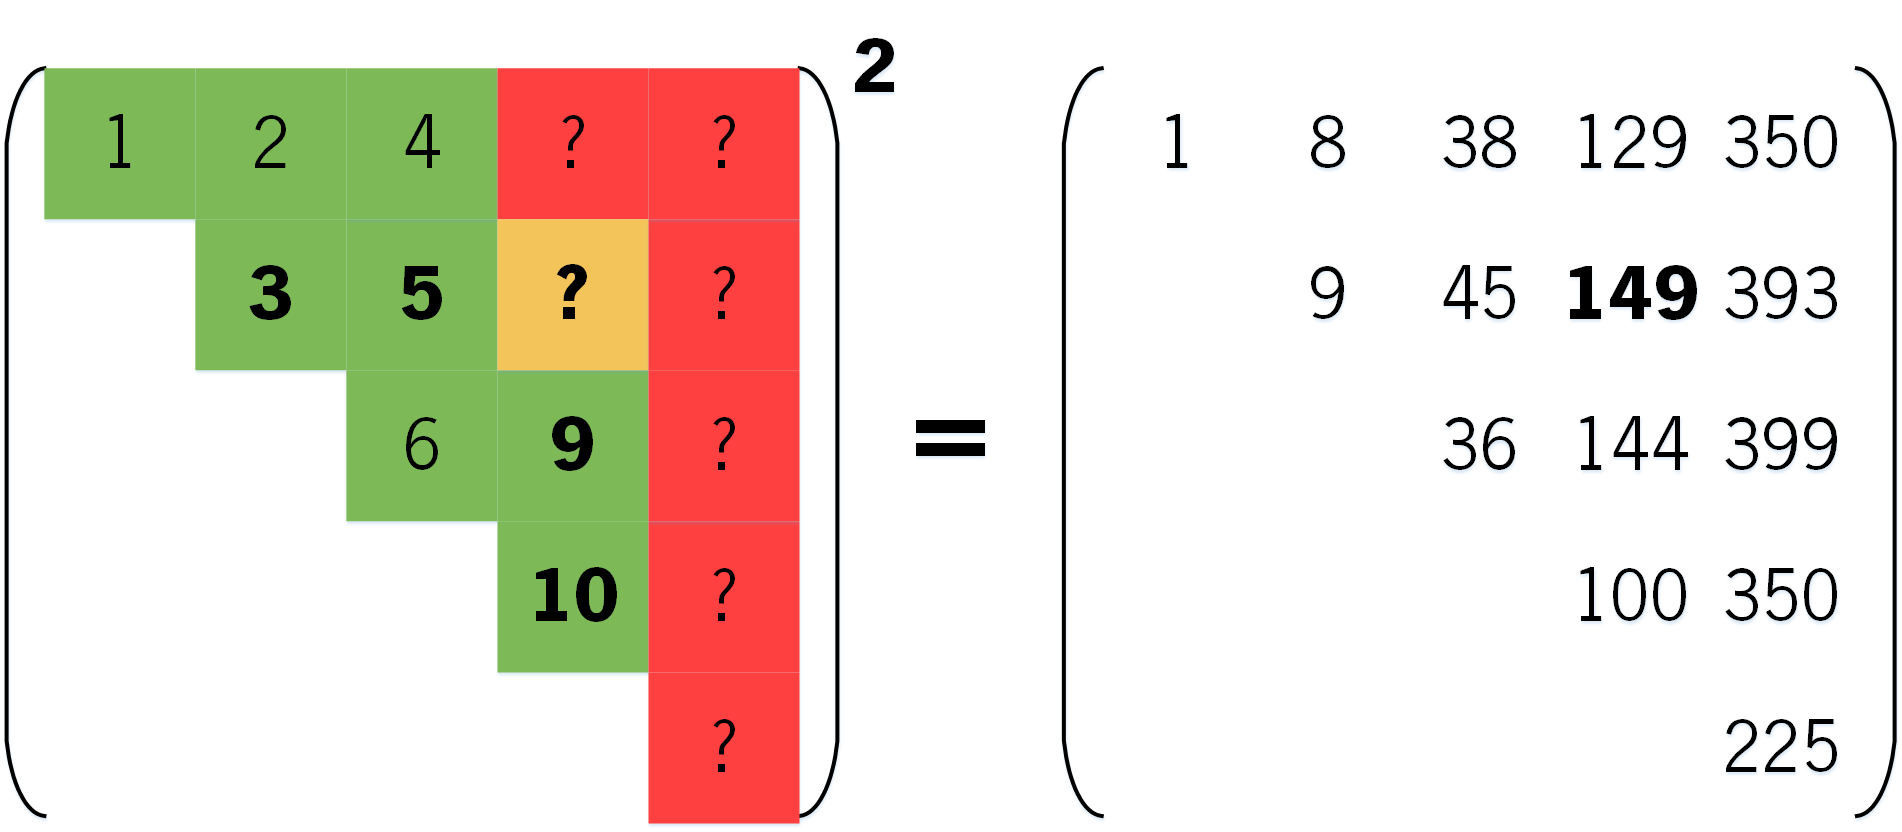
\includegraphics[height=0.16\textheight]{assets/images/case/column.png}
			\caption{Column strategy}
		\end{subfigure}
		\begin{subfigure}{\textwidth}
			\centering
			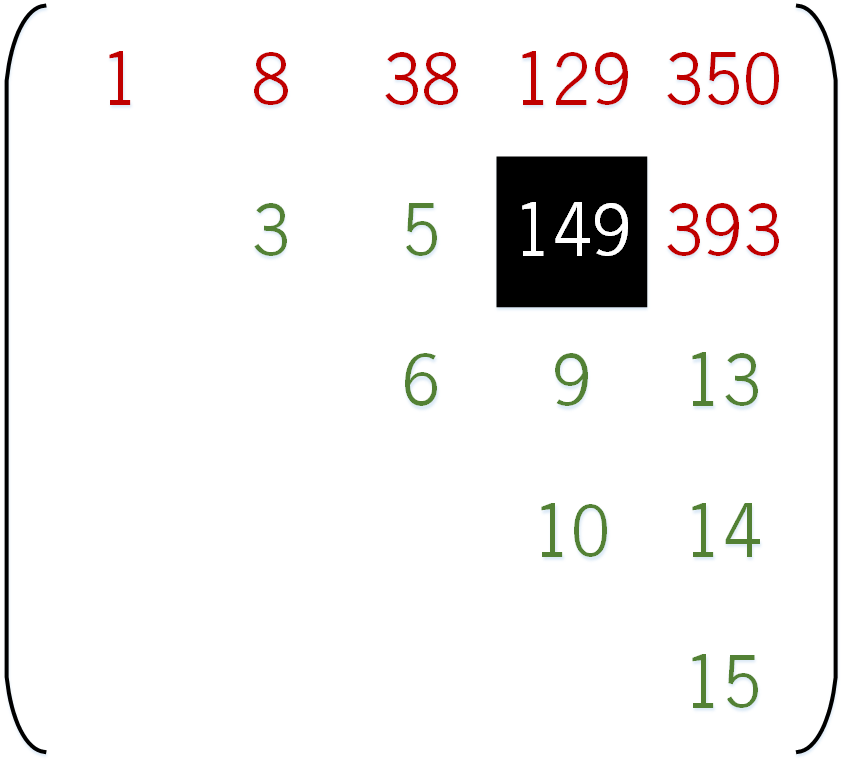
\includegraphics[height=0.16\textheight]{assets/images/case/row.png}
			\caption{Row strategy}
		\end{subfigure}
		\begin{subfigure}{\textwidth}
			\centering
			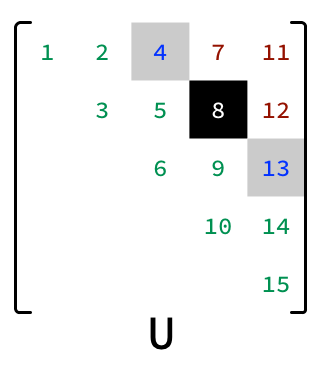
\includegraphics[height=0.16\textheight]{assets/images/case/diagonal.png}
			\caption{Diagonal strategy}
		\end{subfigure}
		\addtolength\belowcaptionskip{-0.5cm}
		\caption[Element/block dependencies and strategies for computing the matrix square root]{Element/block dependencies and strategies for computing the matrix square root: green is solved, red has unsolved dependencies, yellow is ready to be computed next}
	\end{figure}
\end{document}
